
\section{Questions de recherche}

Un éditeur de textes tel que \emph{Microsoft Word}~\cite{word} ou
\emph{Emacs}~\cite{emacs} permet à un utilisateur de créer et d'éditer un
document. Un éditeur de texte collaboratif temps réel~\cite{ellis1991groupware}
étend la rédaction d'un document à un groupe d'utilisateurs. Chacun possède son
éditeur, voit les modifications effectuées par ses collaborateurs sur le
document, effectue ses propres changements en insérant ou en supprimant du
contenu. La mise en place de ces fonctionnalités requière
\begin{inparaenum}[(i)]
\item un moyen de communication entre les éditeurs fonctionnant sur des machines
  potentiellement distantes;
\item un moyen de représenter les documents en mémoire de telle sorte que tous
  les éditeurs affichent un même document lorsqu'ils ont reçu les mêmes
  modifications~\cite{burckhardt2014replicated, shapiro2011conflict}.
\end{inparaenum}

\begin{figure}
  \begin{center}
    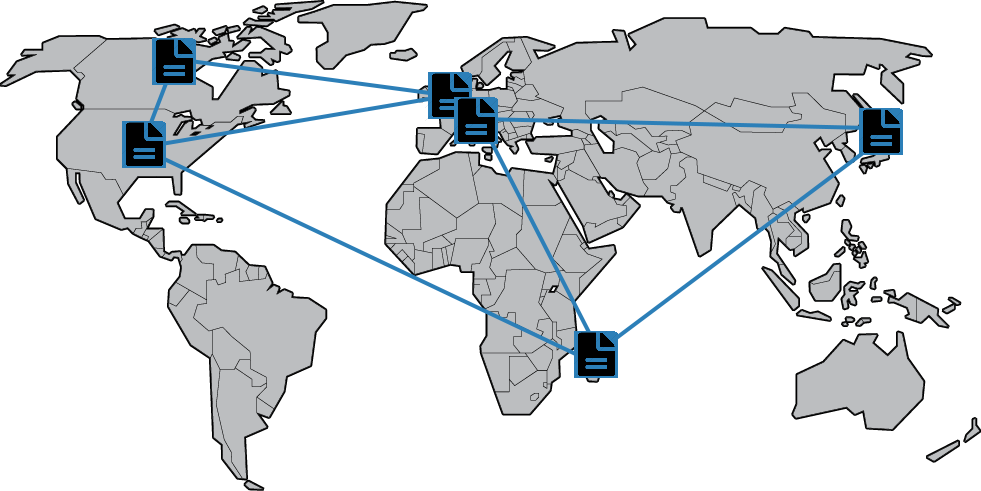
\includegraphics[width=0.85\textwidth]{img/world.png}
    \caption[Édition collaborative décentralisée]{\label{intro:img:world}Édition
      collaborative décentralisée.}
  \end{center}
\end{figure}

La figure~\ref{intro:img:world} présente une session d'édition comprenant 6
auteurs répartis à travers le monde. Afin d'augmenter la disponibilité du
document et de diminuer le temps de réponse lors d'une modification, les
éditeurs collaboratifs actuels suivent le principe de la réplication
optimiste~\cite{saito2005optimistic}. Chaque éditeur collaboratif possède une
copie locale du document.  Lorsque l'utilisateur effectue une modification, elle
est directement répercutée sur sa copie avant d'être envoyée au reste des
éditeurs où elle est intégrée.

% \begin{figure}
%   \begin{center}
%     \begin{tikzpicture}[scale=1.2]

\newcommand\X{25pt}
\newcommand\Y{20pt}

\newcommand\LIGHTGRAY{gray!20}
\newcommand\MEDIUMGRAY{gray!40}

\small
%% communication
\draw[rounded corners=2mm, color=\MEDIUMGRAY, fill=white](0pt, 0pt)+(-4*\X,-\Y)rectangle+(4*\X,\Y);
\draw(4*\X, \Y)node[anchor=north east]{\textbf{\DARKBLUE{communication}}};

\draw ( -3*\X, -0*\Y ) node[anchor=west]{\emph{send and receive changes}};

\small
%% causality
\draw[rounded corners=2mm, color=\MEDIUMGRAY, fill=\LIGHTGRAY](0pt, -2*\Y)+(-4*\X,-\Y)rectangle+(4*\X,\Y);
\draw(4*\X, -\Y)node[anchor=north east]{\textbf{causality}};

\draw( -3*\X, -2*\Y) node[anchor=west]{\emph{track causal relations between changes}};

\small
%% sequence structure
\draw[rounded corners=2mm, color=\MEDIUMGRAY, fill=white](0pt, -4*\Y)+(-4*\X,-\Y)rectangle+(4*\X,\Y);
\draw(4*\X, -3*\Y)node[anchor=north east, align=right]
{\DARKBLUE{\textbf{sequence}}\\\DARKBLUE{\textbf{structure}}};

\draw( -3*\X, -4*\Y) node[anchor=west]{\emph{maintain consistent documents}};

\small
%% gui
\draw[rounded corners=2mm, color=\MEDIUMGRAY, fill=\LIGHTGRAY](0pt, -6*\Y)+(-4*\X,-\Y)rectangle+(4*\X,\Y);
\draw(4*\X, -5*\Y)node[anchor=north east, align=right]
{\textbf{graphical}\\\textbf{user}\\\textbf{interface}};

\draw( -3*\X, -6*\Y) node[anchor=west]{\emph{provide visual cue for interactions}};

\end{tikzpicture}
%     \caption[Architecture des éditeurs collaboratifs]
%     {\label{intro:fig:architecture} Architecture en 4 couches des éditeurs
%       collaboratifs.}
%   \end{center}
% \end{figure}

% La figure~\ref{intro:fig:architecture} montre l'architecture d'un éditeur
% collaboratif constituée de quatre parties :
% \begin{inparaenum}[(i)]
% \item l'interface homme-machine qui constitue le lien entre l'utilisateur et son
%   document, 
% \item la structure de données représentant le document partagé,
% \item la structure de causalité qui permet d'ordonner les changements effectués
%   sur le document,
% \item la couche réseau qui permet de disséminer les changements effectués sur le
%   document.
% \end{inparaenum}
% Aucune de ces couches ne doit empêcher le passage à l'échelle de l'application.
% Cela concerne aussi bien le nombre d'utilisateurs, la taille des documents, la
% fréquence des changements et la durée avant laquelle ils sont intégrés.

L'utilisation des structures de données ``classiques'' telles que les listes
n'est pas directement possible du fait de la latence entre les
collaborateurs. Par exemple, si un auteur insère un caractère en début de document
pendant qu'un autre supprime un caractère au même endroit, le premier auteur
risque, à tort, de voir supprimé le caractère qu'il vient d'insérer. Afin d'éviter
de telles situations, de nouvelles structures et de nouveaux algorithmes doivent
être employés.

Une première famille d'approches consiste à transformer les arguments de
l'opération afin qu'elle considère les opérations intégrées
concurremment~\cite{sun1998operational}. Dans l'exemple précédent, lors de
l'intégration de la suppression par le premier éditeur, celui-ci doit se rendre
compte qu'un caractère a été ajouté en tête concurremment. Il doit donc modifier
les arguments de l'opération reçue afin que le second caractère soit supprimé,
et non plus le premier. Détecter ces cas nécessite de communiquer, avec chaque
opération, des données dont la croissance linéaire empêche au groupe d'éditeurs
d'atteindre de large dimensions~\cite{charronbost1991concerning,
  sun2009contextbased}.

Une seconde famille d'approches consiste à utiliser des structures de données
dont les opérations sont commutatives~\cite{shapiro2011conflict}. Pour que les
opérations commutent, ces approches associent à chaque caractère un identifiant
unique et immuable.

\paragraph{Les identifiants non supprimables~\cite{oster2006data}.} L'opération
de suppression de caractères se contente de cacher le caractère ciblé à
l'utilisateur. Afin de purger la structure des identifiants cachés et ainsi
conserver de bonnes performances, un protocole de ramasse-miettes
réparti~\cite{abdullahi1998garbage} doit être exécuté
régulièrement. Malheureusement, cela s'avère extrêmement
coûteux~\cite{abdullahi1998garbage}.

\paragraph{Les identifiants de taille variable~\cite{weiss2009logoot}.} Les
identifiants sont des listes dont la taille, définie à la génération, peut
grandir très rapidement~\cite{weiss2009logoot}. Cette croissance impacte
négativement les performances du système. Pour y remédier, un protocole de
relocalisation des identifiants doit être exécuté
régulièrement~\cite{zawirskiasynchronous}. Malheureusement, ces protocoles
reviennent à obtenir un consensus dans un contexte réparti. Leur coût s'avère
également très élevé~\cite{mostefaoui2015signature}.

Cela pose la première question de recherche : \textbf{Afin d'éviter tout
  protocole additionnel de relocalisation des identifiants, comment allouer ces
  identifiants de sorte que leur taille soit directement sous-linéaire?}

%%et des canaux de communication avec des
%%éditeurs distants. Une opération effectuée par l'auteur localisé aux États-Unis
%%peut transiter par Madagascar avant de parvenir à l'éditeur Japonais. Une
%%latence entre emission

Pour converger vers des documents identiques, tous les changements doivent
parvenir à tous les éditeurs. Par conséquent, un réseau superposé doit être mis
en place afin de permettre une communication fiable d'un éditeur à l'autre.  La
figure~\ref{intro:img:world} montre que chaque éditeur est connecté à d'autres
éditeurs -- ses voisins -- possédant une réplique du document. Ici, l'éditeur
localisé aux États-Unis communique avec les éditeurs canadien, français et
malgache. Chaque éditeur participe activement au bon fonctionnement du
système. Une opération émise par ce premier peut transiter par l'éditeur
localisé à Madagascar avant de parvenir à l'éditeur japonais.  Les changements
parviennent à tous les éditeurs par transitivité~\cite{birman1999bimodal}.  La
taille des voisinnages est déterminante. En effet, lorsqu'elle augmente, le
trafic généré augmente au risque de dépasser les capacités d'émission des
éditeurs; lorsqu'elle diminue, les changements risquent de ne plus parvenir à
tous les éditeurs.

Afin de configurer la taille de cet ensemble idéalement~\cite{erdos1959random},
le développeur doit connaître le nombre de collaborateurs que l'éditeur
collaboratif doit supporter. Malheureusement, celui-ci varie, que ce soit
pendant la durée de la collaboration, e.g., un cours de formation en ligne
(\emph{MOOC})~\cite{breslow2013studying} voit sa population fluctuer selon
l'intérêt qu'il suscite; ou entre deux documents, e.g., un document créé pour un
événement de grande ampleur n'a pas la même audience que celle d'un rapport de
projet écrit par des étudiants.

Cela pose la seconde question de recherche : \textbf{Comment adapter
  efficacement le voisinage de chaque éditeur au nombre fluctuant de
  collaborateurs?}

%%\paragraph{QR A.} \textbf{Afin d'ajuster le trafic à la session d'édition,
%%  comment adapter efficacement le voisinage de chaque éditeur aux fluctuations
%%  des réseaux?}



%%% Local Variables:
%%% mode: latex
%%% TeX-master: "../../paper"
%%% End:
